\chapter{实验测试与数据分析}
\label{cha:chapter6}
为了保证低功耗海洋传感器集成系统能够在低功耗指标下长期稳定的运行在海底环境中,在完成搭载平台的软硬件设计之后,需要对该平台进行集成实验测试,以保证平台的稳定性和可靠性。首先在实验室进行了模拟实验,对硬件平台的各部分功能模块进行了实验验证,对其中存在的错误和缺陷及时修改并补充,以达到所需的要求。之后将该平台在布放在海洋环境以完成实际的试验,最终实现海洋水文数据的采集和保存等功能。

\section{室内环境实验}
在将各个软硬件部分进行组装集成后,在实验室进行基本的功能和性能测试,以及低功耗、稳定性和可靠性测试。

主要是对传感器电源供电管理功能测试,包括上电和断电等功能、并对各传感器下达采样命令进行数据采集功能检测、传感器正常工作时的状态监测,包括电压和温度监控等、以及平台的整体运行性能等测试。通过多次实验证明,各传感器连接控制模块电压正常,能够为传感器做到正常上断电以及状态信息实时反馈,同时对传感器进行相关配置并下达采样命令后,将进行数据采集任务,通过串口将数据传送给微处理器,再对数据进行解析处理,最后通过TF卡将数据保存或者通过USB接口将数据回收。系统不需要进行采样时,微控制器进入低功耗模式,此时整个系统处于休眠状态。对于仅依靠于电池组供电的系统来说,休眠状态大大节省了电池电量,延长了系统在海洋环境下的生存时间。

在实验室经过30天稳定运行后,对于传感器电源管理、低功耗模式以及数据采集等功能均能正常平稳进行,平台的整体功能及性能基本可以达到投放条件。同时经过反复实验检测,对其中出现的问题做到及时反馈分析并解决,并且对平台的软硬件部分功能进行优化和改进设计,以最终满足整体布放和业务化运行条件。

水密控制舱和系统平台框架搭建完成后的室内环境测试实验具体分为三个部分:耗电测试、命令测试和数据测试。
\subsection{耗电测试}
为了测试系统具体的低功耗性能指标,通过预留的USB接口连接到个人电脑,使用串口调试助手,给微处理器发送系统交互的命令进行电源控制,在供电电压在12V的情况下,采用高精度数字直流电源,记录各部件耗电情况。通过微处理器控制给所有的外部部件断电,测得的即是MCU单元电流,然后分别控制MCU进入活跃状态和低功耗状态,得到不同工作模式下MCU单元的电流,依次控制给各个部件上电,测量其电流大小,各部件耗电电流如表格~\ref{tab:各部件耗电情况}所示。

%\newcommand{\tabincell}[2]{\begin{tabular}{@{}#1@{}}#2\end{tabular}}  
%表格自动换行
\begin{table*}[ht]
\caption{各部件耗电情况}
  \label{tab:各部件耗电情况}
\centering
    \begin{tabular}{|c|c|c|c|}
        \toprule
 {\bf 部件名称}&{\bf 部件功耗/mA} & {\bf 每小时工作时长/s} & {\bf 每日平均功耗/Ah}\\    
%\bf表示字体加粗
        \hline
 {活跃状态MCU单元}&{5mA} & {3600}&{0.12}\\      
%\bf表示字体加粗
        \hline
 {低功耗状态MCU单元}&{可忽略} & {3600}&{可忽略}\\      
%\bf表示字体加粗
        \hline
 {MAX232CSE芯片}&{1mA} & {3600}&{0.024}\\      
%\bf表示字体加粗
        \hline
 {串口拓展芯片WK2124}&{3mA} & {3600}&{0.072}\\      
%\bf表示字体加粗
        \hline
 {时钟芯片DS3234}&{2mA} & {3600}&{0.036}\\      
%\bf表示字体加粗
        \hline
{CH340E芯片}&{1mA} & {3600}&{0.024}\\      
%\bf表示字体加粗
        \hline
{TF卡模块}&{30mA} & {60}&{0.012}\\      
%\bf表示字体加粗
        \hline
{AML系列传感器(温盐)}&{72mA} & {60}&{0.029}\\      
%\bf表示字体加粗
        \hline
{溶解氧传感器}&{48mA} & {60}&{0.019}\\      
%\bf表示字体加粗
        \hline
    \end{tabular}
\end{table*}
表格~\ref{tab:各部件耗电情况}列举的各部件耗电占据了系统能源消耗绝大部分,其余的一些外部部件,由于耗电非常低,几乎可以对其进行忽略。按照目前完成的实验室测试数据,系统集成4个AML系列海洋传感器和1个溶解氧传感器,每个小时传感器采集一分钟数据,然后进行数据存储的情况下,一天内的总功耗大约是0.442/Ah,本设计使用七节锂电池串联组作为接入电源,锂电池的容量为95Ah,运行天数是215天。实际的应用中,海洋传感器集成数量和采集周期的不同,都会导致系统有效工作时长会发生变化。
\subsection{命令测试}
进行命令测试,目的是确保设备的功能性、稳定性。一般向海洋传感器长时间反复发送一些常用的命令,可以检查出电气连接和功能是否有问题。

1)查看目前串口通信的传感器探头类型,可以发送VERSION命令,串口将会接收到传感器反馈回来的版本信息如图~\ref{fig:VERSION命令}所示。

\begin{figure*}[ht]
    \centering
	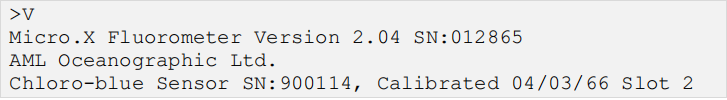
\includegraphics[width=1\textwidth]{fig/VERSION命令.png}
	\caption{VERSION命令}
	\label{fig:VERSION命令}
\end{figure*}

2)一些重要的设置命令测试,比如设置串口的波特率和传感器的采样频率。

串口通信必须约定双方使用相同的波特率。设置波特率的命令是SET DETECT ab,b可以是1到9的数字。 

数字所对应的波特率如下所示:

\begin{lstlisting}
1 = 600
2 = 1200
3 = 2400
4 = 4800
5 = 9600
6 = 19200
7 = 38400
8 = 57600
9 = 115200
\end{lstlisting}

每次在使用串口通信的波特率配置时,根据系统所需要的波特率,去找到数字所对应的波特率即可。如图~\ref{fig:波特率设置命令}所示的命令表示将串口波特率设置为38400(b=7)。在本次设计中一般使用9600的波特率,直接将b代表的数字改成6就可完成波特率设置。

\begin{figure*}[ht]
    \centering
	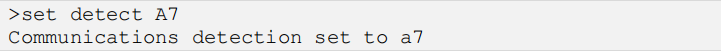
\includegraphics[width=1\textwidth]{fig/波特率设置命令.png}
	\caption{波特率设置命令}
	\label{fig:波特率设置命令}
\end{figure*}

采样率是传感器配置的关键参数之一,决定了传感器的采样速率,AML系列的海洋传感器具有采样速率高的特点,最高速率可达每秒25个样本。SET SAMPLE RATE n t(简写为SET S)是设置采样率的命令,其中n t有不同的表示方法,这样对于用户使用来说更加灵活,既可以设置为采样率,也可以用采样周期来表示,如下所示:

\begin{lstlisting}
n /S:将采样率设置为每秒n个样本。
n /M:将采样率设置为每分钟n个样本。
n /H:将采样率设置为每个小时n个样本。
n S:样本的采样周期设置为n秒。
n M:样本的采样周期设置为n分钟。
n H:样本的采样周期设置为n小时。
\end{lstlisting}

如图~\ref{fig:采样率设置命令}所示的命令分别表示样本采样周期为一秒和采样率为每秒一个样本。

\begin{figure*}[ht]
    \centering
	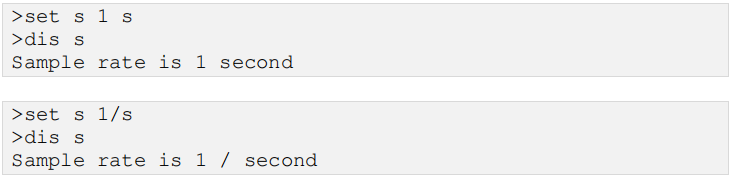
\includegraphics[width=1\textwidth]{fig/采样率设置命令.png}
	\caption{采样率设置命令}
	\label{fig:采样率设置命令}
\end{figure*}

3)接下来测试采样命令SCAN(简写为S)和MONITOR(简写为M).它们的区别是:SCAN是输出一次数据扫描,MONITOR是流数据按设置的采样率输出。

\begin{figure*}[ht]
    \centering
	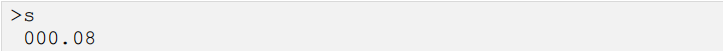
\includegraphics[width=1\textwidth]{fig/SCAN命令.png}
	\caption{SCAN命令}
	\label{fig:SCAN命令}
\end{figure*}

如图~\ref{fig:SCAN命令}所示,SCAN命令进行了一次采样。

\begin{figure*}[ht]
    \centering
	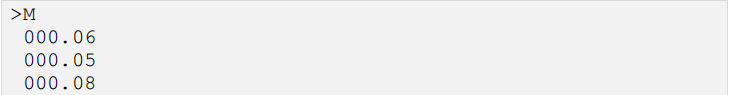
\includegraphics[width=1\textwidth]{fig/MONITOR命令.png}
	\caption{MONITOR命令}
	\label{fig:MONITOR命令}
\end{figure*}

如图~\ref{fig:MONITOR命令}所示,MONITOR命令进行按采样率进行连续采样。

命令测试主要是为了测试系统功能性和稳定性,在功能性上使用串口调试助手等工具对低功耗海洋传感器系统反复下达控制指令,比如微处理工作模式选择和切换以及海洋海洋传感器进行上电、断电、命令下达等功能性测试,以上操作都能准确执行。在进行稳定性的测试过程中,整个系统的软硬件平台均能连续稳定工作30天以上,符合稳定性测试要求。

\subsection{数据测试}
数据测试的主要作用是保证系统通过海洋传感器采集而来的数据具有现实意义和研究价值。室内环境,要测试微处理器控制板在连接不同的传感器探头情况下,采集水文数据,其数据的有效性。利用控制变量的实验方法对采样数据进行对比分析。

1.对Smart Turbidity(浊度)传感器进行测试。

测试方法:用杯子取半杯自来水,水量恰好满过传感器,进行数据采样,如图~\ref{fig:浊度传感器测量自来水}所示。
\begin{figure*}[ht]
    \centering
	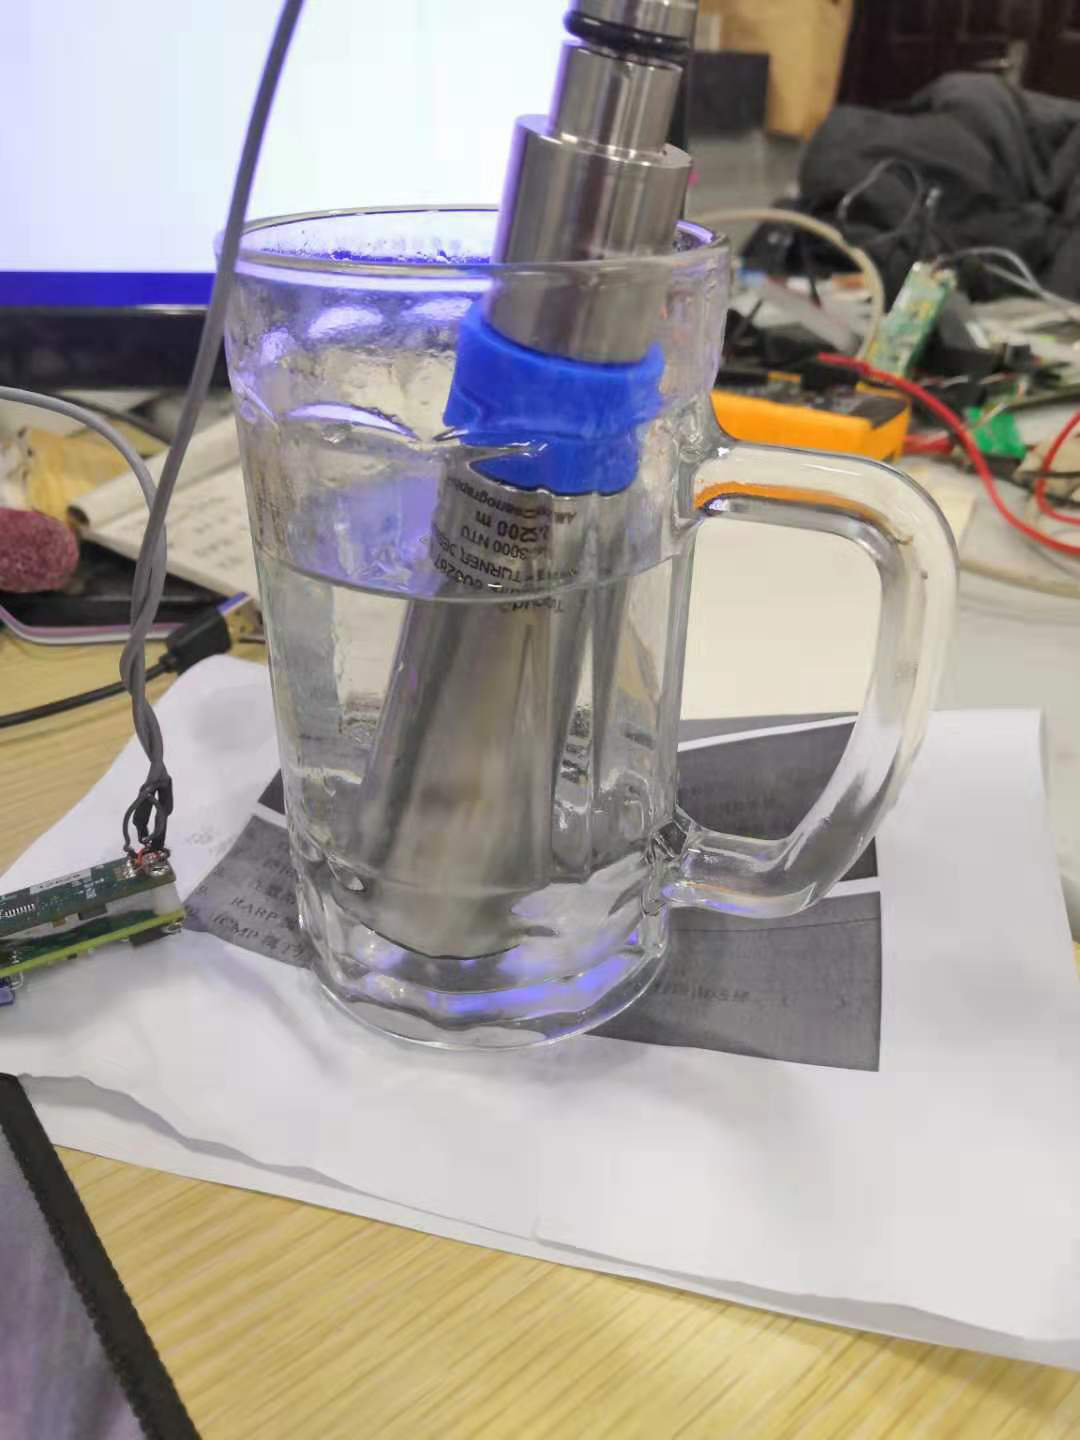
\includegraphics[width=0.4\textwidth]{fig/浊度传感器测量自来水.png}
	\caption{浊度传感器测量自来水}
	\label{fig:浊度传感器测量自来水}
\end{figure*}

之后往水杯中加入几毫升牛奶,摇晃均匀后采样,如图~\ref{fig:浊度传感器测量混有牛奶的自来水}所示。

\begin{figure*}[ht]
    \centering
	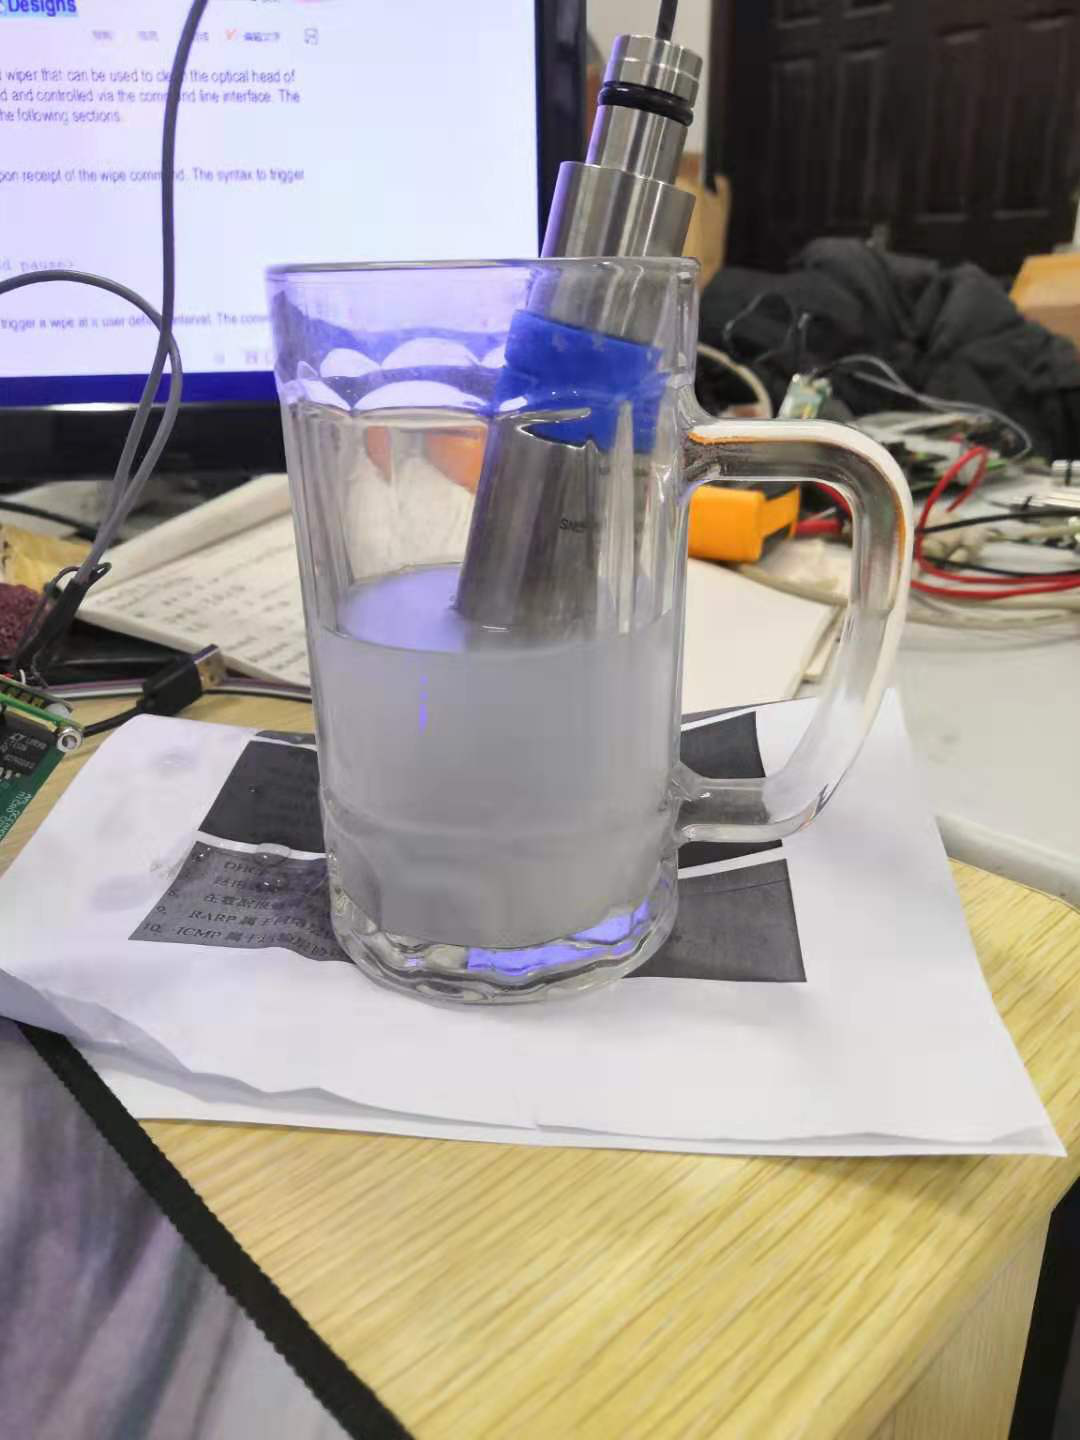
\includegraphics[width=0.4\textwidth]{fig/浊度传感器测量混有牛奶的自来水.png}
	\caption{浊度传感器测量混有牛奶的自来水}
	\label{fig:浊度传感器测量混有牛奶的自来水}
\end{figure*}

智能浊度传感器在监测时传输两个数据通道,测量通道和状态通道。测量通道包含传感器收集的测量数据。由于智能浊度传感器配有驱动雨刷,可用于清洁探头的气泡、微生物或碎片。状态通道指示每次测量是否可靠。测量可能已被雨刷的活动损坏。状态为0表示可靠数据,而状态为1表示测量可能受到雨刷活动的强烈影响。

表~\ref{tab:浊度}列举了智能浊度传感器在自来水和牛奶溶液下分别三次采样数据,在不受雨刷影响下对两种溶液所测量得到的数据差异很大,同一溶液之间的三次采样误差很小。
\begin{table}[ht]
\caption{浊度传感器对两种不同浊度溶液的三次采样}
\label{tab:浊度}
\centering
    \begin{tabular}{|c|c|c|c|}
        \hline
        \diagbox{溶液}{采样编号} & 第一次 & 第二次&第三次 \\   
        %斜线命令语句
        \hline
        自来水 &0005.05 0&0005.04 0 &0005.14 0\\
         \hline
        混有牛奶的自来水 & 0339.35 0 &0339.57 0&0339.36 0\\
         \hline
    \end{tabular}
\end{table}

2.对CT(盐度和温度)传感器进行测试。

测试方法:用杯子取半杯自来水,水量恰好满过传感器,进行数据采样,然后将杯子内的自来水倒出少许,换成热水采样,最后将杯子内的自来水换成标准海水采样。由于CT传感器具有两种参数,设置了两组对照试验来对比。

CT传感器在监测时传输两个数据通道。一个通道输出电导率数据(反应出盐度参数),另一个通道输出温度数据。

\begin{table}[ht]
\caption{CT传感器对三种不同溶液的三次采样}
\label{tab:CT•Xchange}
\centering
    \begin{tabular}{|c|c|c|c|}
        \hline
        \diagbox{溶液}{采样编号} & 第一次 & 第二次&第三次 \\   
        %斜线命令语句
        \hline
        自来水 &00.967 19.860&00.965 19.860&00.967 19.858\\
         \hline
        温水 & 00.909 23.897&00.911 23.894&00.912 23.892\\
         \hline
        标准海水 & 42.356 19.951&42.361 19.955&42.362 19.959\\
         \hline
    \end{tabular}
\end{table}

表格~\ref{tab:CT•Xchange}列举了CT传感器对自来水、温水、海洋三种不同溶液的三次采样数据,可以看到自来水和温水之间有温度数据上的差异,在采样的同时,使用温度计对两种溶液温度进行了测定,在温度数据上与CT传感器采集温度数据差异很小,而自来水和标准海水之间在盐度数据上的差异较大,这符合常规认知。


3.对Smart pH传感器进行测试。
测试方法:用杯子取半杯自来水,水量将将满过传感器。将杯子内的自来水换成标准海水。对比不同PH值的水采样数据的差异。

\begin{table}[ht]
\caption{Smart pH传感器对两种不同溶液的三次采样}
\label{tab:PH}
\centering
    \begin{tabular}{|c|c|c|c|}
        \hline
        \diagbox{溶液}{采样编号} & 第一次 & 第二次&第三次 \\   
        %斜线命令语句
        \hline
        自来水 &06.40&06.3 & 06.2\\
         \hline
        标准海水 & 06.7 &06.7&06.7\\
         \hline
    \end{tabular}
\end{table}

从表格~\ref{tab:PH}中看到,采样的自来水和标准海洋的PH数据差异并不大,经过查阅互联网资料发现这两种溶液PH值是有可能出现相近的情况。

4.对Smart Chlorophy (叶绿素)传感器进行测试。
测试方法:用杯子取半杯自来水,水量将将满过传感器。将杯子中的自来水换成从河道取来的河水。对比不同叶绿素含量的水采样数据的差异。

\begin{table}[ht]
\caption{Smart Chlorophy传感器对两种不同溶液的三次采样}
\label{tab:chl}
\centering
    \begin{tabular}{|c|c|c|c|}
        \hline
        \diagbox{溶液}{采样编号} & 第一次 & 第二次&第三次 \\   
        %斜线命令语句
        \hline
        自来水 &000.26&000.24 & 000.26\\
         \hline
        河道水 & 020.50 &021.55&021.65\\
         \hline
    \end{tabular}
\end{table}

从表格~\ref{tab:chl}中看到,河道水中叶绿素的含量比自来水丰富很多,河道水的叶绿素反应了藻类的浓度较高,自来水经过消毒,其藻类浓度自然很低。

5.对UV灯进行测试。
测试方法:设置亮灭时间分别为一分钟和两分钟,然后用手机秒表计数。
\begin{table}[ht]
\caption{UV灯定时闪烁测试}
\label{tab:UV}
\centering
    \begin{tabular}{|c|c|c|c|}
        \hline
        \diagbox{时长}{采样编号} & 第一次 & 第二次&第三次 \\   
        %斜线命令语句
        \hline
        60S &\tabincell{c}{灭-59.45s  \\ 亮-60.15s}&\tabincell{c}{灭-59.65s \\ 亮-60.25s}&\tabincell{c} {灭-59.55s \\  亮-60.15s}\\
         \hline
        120S&\tabincell{c}{灭-119.75s \\   亮-119.15s}&\tabincell{c}{灭-120.65s \\  亮-120.25s}& \tabincell{c}{灭-119.55s \\  亮-120.15s}\\
         \hline
    \end{tabular}
\end{table}

表格~\ref{tab:UV}通过秒表计时时间与设置的闪烁时间进行对比,可知UV灯的功能是基本正常的。
\section{室外环境实验}
室内环境实验测试完成后,为了确保系统在室外海域环境下能达到长期稳定运行的要求,接下来需进行外部环境测试。为了模拟海洋的实际环境提高实验的仿真性,对低功耗海洋传感器集成系统进行了为期30天的浅海选址、布放、回收的试验。经过为期30天的浅海测试分析,低功耗海洋传感器集成系统的各部分软硬件都能稳定的工作,传感器进行能源管理、数据采集和命令下达控制,修改各传感器采样配置方案等操作均正常工作。综上所述,系统已达到长期稳定运行的要求。外部环境布放如图~\ref{fig:外部环境测试效果图}所示。

\begin{figure*}[ht]
    \centering
	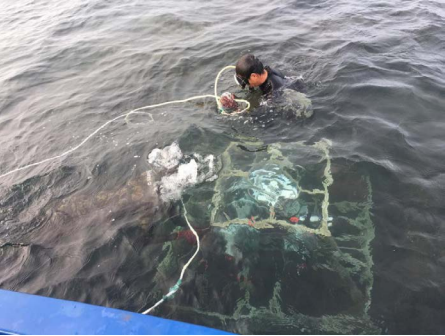
\includegraphics[width=0.7\textwidth]{fig/外部环境测试效果图.png}
	\caption{外部环境布放图}
	\label{fig:外部环境测试效果图}
\end{figure*}

\section{实验数据分析}
多参数水质仪采样的数据包括水位、海水温度、盐度、溶解氧、叶绿素、浊度、PH。经过30天的布放使用和观察,现对第1周采集的数据进行汇总和分析,大致总结了如下数据的变化趋势。

浅海测试海域的潮汐变化以潮周期变化为主,最高水位18m左右,最低水位15m左右,高低水位差3m左右,平均水位在16.5m,变化范围在0.5-1.3m之间。经过第1 周的潮汐高低的水位变化的观察,存在高水位较高、最低水位较高的现象,故将浅海海域判定为不正规全日潮类型。在水温监测方面,7天的时间整体气温呈明显的下降趋势,存在3天时间有小幅升温。观测过程中平均水温29.1℃,平均日温差 12℃。在盐度监测方面,由于浅海海域温度相对稳定,近海岸海水盐度变化较小,7天观测期未出现明显波动。观测时间段内平均盐度为32.06,标准差在0.0016,盐度较为均匀。在溶解氧监测方面,平均浓度为6.46mg/L,日变化幅度在0.3-0.5mg/L之间,标准差为0.0061mg/L。在叶绿素监测方面,在观测期间的第4天出现峰值,其余时间变化幅度相对稳定,叶绿素浓度平均值为0.232μg/L,浓度标准差约为0.0016μg/L。在浊度监测方面,观测值在后3天增长趋势较大,7天内的浊度平均值为0.873,标准差位0.0652,相对于温度、盐度、叶绿素三个数据浊度变化幅度较大。在PH值监测方面,在第4日至第7日上升幅度较大,7天内PH平均值为8.213,标准差为0.0006。以上信息汇总如图~\ref{fig:测试数据}所示。

\begin{figure*}[ht]
    \centering
	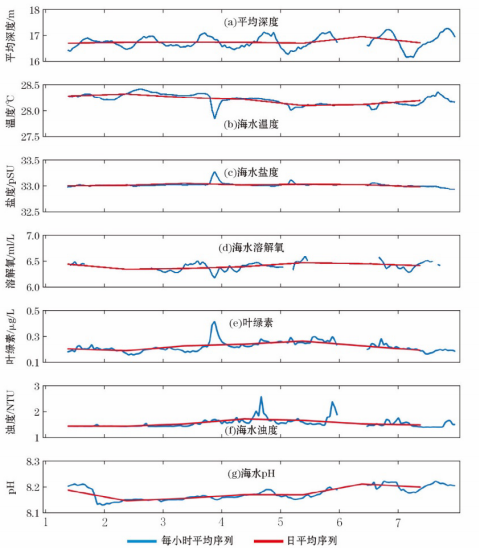
\includegraphics[width=1\textwidth]{fig/浅海测试第1周海洋水文数据曲线图.png}
	\caption{浅海测试第1周海洋水文数据曲线图}
	\label{fig:测试数据}
\end{figure*}

\section{本章小结}
在完成系统整体架构设计和系统的软硬件设计后,先后进行了水密控制舱和平台整体框架的组装。为了保证系统实际布放后可以长期稳定的运行,依次进行系统通信速率测试、功能稳定测试的室内环境实验和为期30天浅海的外部环境实验,经测试和分析海洋水文数据、海洋动力数据,初步认定低功耗海洋传感器集成系统符合功能性和稳定性的要求,可在海洋环境布放设备并陆续开展实际数据采集工作。